\documentclass[11pt]{article}

\usepackage[review]{acl-style-files/acl}

\usepackage{times}
\usepackage{latexsym}
\usepackage[T1]{fontenc}
\usepackage[utf8]{inputenc}
\usepackage{microtype}
\usepackage{inconsolata}
\usepackage{graphicx}
\usepackage{booktabs}
\usepackage[table]{xcolor}
\usepackage{amsmath}
\usepackage{multirow}
\usepackage{enumitem}
\usepackage{url}
\usepackage[capitalize,noabbrev]{cleveref}

\newcommand{\ours}{EvoClawBench}
\newcommand{\baseline}{\textsc{Baseline}}
\newcommand{\preskill}{\textsc{PreSkill}}
\newcommand{\postskill}{\textsc{PostSkill}}

\title{\ours{}: Benchmarking Self-Evolving Agents That Create and Reuse Skills at Runtime}

\author{
  Anonymous ACL submission
}

\begin{document}
\maketitle

\begin{abstract}
User-defined skills have rapidly become a practical mechanism for specializing LLM agents to recurring tasks.
As foundation models improve, the ecosystem is expanding quickly: 84{,}192 skills were created within 136 days.
This growth raises a new evaluation question: can an LLM agent improve itself at runtime by creating reusable skills, and do those skills actually improve later task execution?
We present \textbf{\ours{}}, a benchmark for measuring skill self-evolution across repeated, tool-using tasks.
\ours{} compares three execution strategies: a no-skill \baseline{} condition, a \preskill{} condition that asks the same agent to author task-specific skills before execution, and a \postskill{} condition that asks the agent to summarize reusable skills from a first run before solving the task again.
The benchmark currently includes 100 tasks spanning data transformation, log analysis, API scaffolding, test generation, configuration migration, code review, document extraction, office automation, finance, legal operations, healthcare administration, procurement and logistics, HR and education, support and product operations, DevOps and SRE, security and privacy, data analytics, research and media, localization and release management, commerce and food operations, facilities and IoT, public-sector audit, CRM, executive operations, and travel/office coordination, and supports multiple agent runtimes including OpenClaw and nanobot.
Our current OpenClaw evaluation runs the hardened suite in local execution with 32 workers, \texttt{mode=all}, and \texttt{openai/MiniMax/MiniMax-M2.7} as the hybrid judge.
Across two valid model runs, direct \baseline{} performance remains below 20\% mean score, showing that the hardened tasks avoid the saturation observed in earlier drafts.
Skill timing is model-dependent: \texttt{openai/gpt-5.4} collapses under \postskill{}, while \texttt{openai/qwen3.6-plus} keeps \postskill{} close to \baseline{} and above \preskill{}.
A third \texttt{openai/deepseek-v4-pro} run is reported only as an invalid audit row because it contains 13 LLM judge failures.
\end{abstract}

\section{Introduction}
\label{sec:intro}

Large language model agents are increasingly deployed as interactive workers that read files, call tools, write code, inspect outputs, and revise their own solutions.
Alongside stronger foundation models, a complementary trend has emerged: users package procedural knowledge into reusable \emph{skills}, typically written as structured markdown documents with optional scripts, templates, and references.
Skills encode task-specific expertise such as how to audit dependencies, generate CI configurations, scaffold APIs, extract tables, or perform domain-specific data analysis.
They are attractive because they are lightweight: a skill can be installed, inspected, edited, and injected into an agent's context without retraining the model.

The skill ecosystem is growing at a speed that outpaces careful evaluation.
Recent reports show that 84{,}192 skills were created within only 136 days \citep{li2026skillsbench}.
This scale suggests a shift from prompt engineering by individual users toward a marketplace of reusable procedural memory.
However, the central question is no longer only whether a human-written skill can help an agent.
If agents are to become long-running assistants, they must also decide when to create skills, what to write into them, and whether those self-authored skills improve later work.

Existing benchmarks do not directly measure this capability.
SWE-Bench and SWE-agent-style evaluations emphasize repository-level software engineering \citep{jimenez2024swebench,yang2024sweagent}.
Terminal-Bench and AppWorld evaluate tool use and command-line or app-world interaction \citep{merrill2026terminalbench,trivedi2024appworld}.
SkillsBench treats skills as first-class artifacts across domains \citep{li2026skillsbench}, but it focuses on evaluating provided skill conditions rather than the agent's ability to create, summarize, and reuse its own skills during a benchmark run.
As a result, there is still no standard testbed for the following question: \emph{Can an LLM agent self-evolve by creating skills that improve its own task performance?}

We introduce \ours{}, a benchmark designed around this question.
\ours{} evaluates an agent on repeated, structured tasks that contain multiple related sub-problems.
This design creates an opportunity for the agent to recognize shared patterns and convert them into reusable skills.
For each task, we compare three strategies.
In \baseline{}, the agent solves the task directly and is forbidden from creating or editing skills.
In \preskill{}, the same model and runtime first create one or more task-specific skills, then a fresh execution workspace solves the task using only those generated skills.
In \postskill{}, the agent first solves the task without skills, receives a compact first-run context containing the prompt, grading summary, output previews, and transcript summary, then writes reusable skills that are copied into a fresh second execution.

This protocol isolates two related but distinct forms of self-evolution.
\preskill{} measures whether an agent can infer a useful reusable procedure before solving a task.
\postskill{} measures whether an agent can distill reusable procedural memory from experience.
Both are compared against \baseline{} under execution-only and end-to-end metrics, so a skill workflow must improve not only task score but also justify its additional token, cost, and time overhead.

\begin{figure*}[t]
\centering
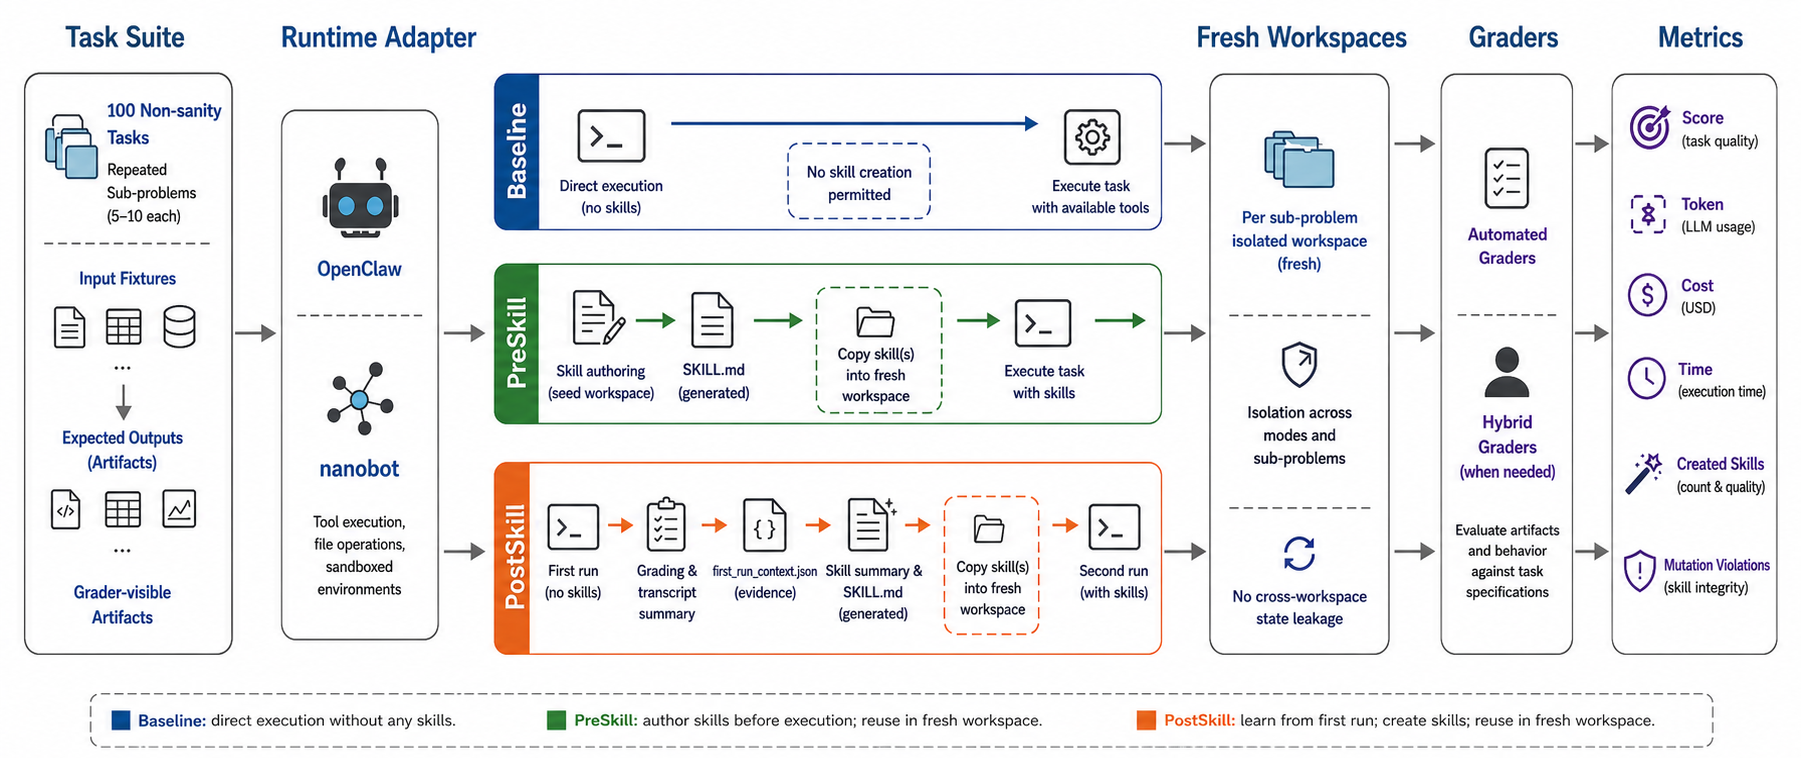
\includegraphics[width=\textwidth]{Figures/fig_overview_imagegen.png}
\caption{Overview of \ours{}. The benchmark runs repeated, fixture-backed tasks through shared runtime adapters, compares \baseline{}, \preskill{}, and \postskill{} execution in fresh workspaces, and reports task quality, efficiency, skill creation, and mutation-integrity metrics.}
\label{fig:overview}
\end{figure*}

Our paper makes the following contributions:
\begin{itemize}[leftmargin=*]
    \item \textbf{Benchmark.} We build \ours{}, a benchmark for evaluating runtime skill self-evolution in LLM agents. It covers 100 tasks with repeated sub-problems, fixtures, automated or hybrid graders, and multiple agent runtimes.
    \item \textbf{Three-mode evaluation protocol.} We formalize \baseline{}, \preskill{}, and \postskill{} conditions, separating execution-only performance from end-to-end workflow cost and detecting skill mutation violations during reuse.
    \item \textbf{Empirical findings.} We provide a current OpenClaw result table showing that the hardened suite keeps valid model baselines below 20\%, and that self-authored skills do not produce monotonic gains. \preskill{} and \postskill{} can both regress relative to \baseline{}, and invalid judge-failure rows must be excluded from capability conclusions.
\end{itemize}

\section{Related Benchmarks and Skill Evaluation}
\label{sec:related}

\paragraph{Agent and software engineering benchmarks.}
Repository-level software engineering benchmarks evaluate whether agents can modify realistic codebases and satisfy executable checks.
SWE-Bench evaluates real GitHub issue resolution \citep{jimenez2024swebench}, while SWE-agent studies agent-computer interfaces for automated software engineering \citep{yang2024sweagent}.
Terminal-Bench focuses on realistic command-line tasks in isolated environments \citep{merrill2026terminalbench}.
AppWorld and $\tau$-Bench broaden the scope to interactive applications and tool-agent-user settings \citep{trivedi2024appworld,yao2025taubench}.
These benchmarks are useful for measuring tool use and task completion, but they do not test whether an agent can write reusable skills at runtime and then benefit from them.

\paragraph{Skill and procedural memory evaluation.}
Skills can be viewed as external procedural memory for agents, related to work on agent skills, procedural memory, and open-ended skill acquisition \citep{anthropic2025skills,fang2025memp,wang2023voyager,xu2026agentskills,wu2026agentskillsmemory}.
SkillsBench is closest to our setting because it evaluates skills as first-class artifacts \citep{li2026skillsbench}.
However, the central object in \ours{} is not only a pre-existing skill.
Instead, \ours{} evaluates the \emph{closed-loop} process in which the same runtime and model being benchmarked must author, summarize, and reuse its own skill artifacts.

\Cref{tab:comparison} summarizes the benchmark position.
\ours{} is designed to expose whether skill self-evolution improves task success after accounting for the full cost of creating and reusing skills.

\begin{table*}[t]
\centering
\small
\caption{Comparison of \ours{} with related benchmarks. ``Skill Create'' indicates whether the benchmark evaluates skills authored by the agent during the benchmark run. ``Reuse Cond.'' indicates an explicit skill-reuse execution condition. ``Multi-runtime'' indicates support for evaluating multiple agent runtimes or claws under the same task suite.}
\label{tab:comparison}
\resizebox{\textwidth}{!}{%
\begin{tabular}{lcccccc}
\toprule
\textbf{Benchmark} & \textbf{Size} & \textbf{Realistic Env.} & \textbf{Skill Create} & \textbf{Reuse Cond.} & \textbf{Multi-runtime} & \textbf{Cost Metrics} \\
\midrule
SWE-Bench \citep{jimenez2024swebench} & 2{,}294 & Yes & No & No & Partial & Partial \\
Terminal-Bench \citep{merrill2026terminalbench} & 200 & Yes & No & No & Yes & Partial \\
AppWorld \citep{trivedi2024appworld} & 750 & Yes & No & No & Yes & Partial \\
$\tau$-Bench \citep{yao2025taubench} & 165 & Yes & No & No & Yes & Partial \\
SkillsBench \citep{li2026skillsbench} & 84 & Yes & No & Yes & Partial & Yes \\
\midrule
\textbf{\ours{}} & \textbf{100} & \textbf{Yes} & \textbf{Yes} & \textbf{Yes} & \textbf{Yes} & \textbf{Yes} \\
\bottomrule
\end{tabular}
}
\end{table*}

\section{\ours{} Construction}
\label{sec:construction}

\ours{} is constructed to test whether an agent can recognize repeated structure across sub-problems and encode that structure as a reusable skill.
The benchmark implementation is organized around task definitions, workspace fixtures, runtime adapters, graders, and metric aggregation.

\subsection{Task Suite}
\label{subsec:tasks}

Tasks are written as markdown files with YAML frontmatter, a natural-language prompt, expected behavior, sub-problem descriptions, grading criteria, and automated or hybrid grading logic.
Each task usually contains five to ten structurally related sub-problems.
This repeated structure is important: it gives the agent a reason to write down a general procedure rather than solve a single isolated instance.

The current task suite covers data transformation, log analysis, API scaffolding, test generation, configuration migration, security review, document extraction, database operations, Excel analytics, web extraction, document generation, data pipelines, email and invoice processing, shell automation, CI generation, dependency audit, environment configuration, metrics anomaly detection, finance operations, legal operations, healthcare administration, procurement and logistics, HR and education, support and product operations, DevOps/SRE, security and privacy, data analytics, research and media, localization and release management, commerce and food operations, facilities and IoT, public-sector audit, CRM and executive operations, and travel/office coordination.
The suite size is 100 tasks and 502 sub-problems after excluding the sanity task.

\begin{figure*}[t]
\centering
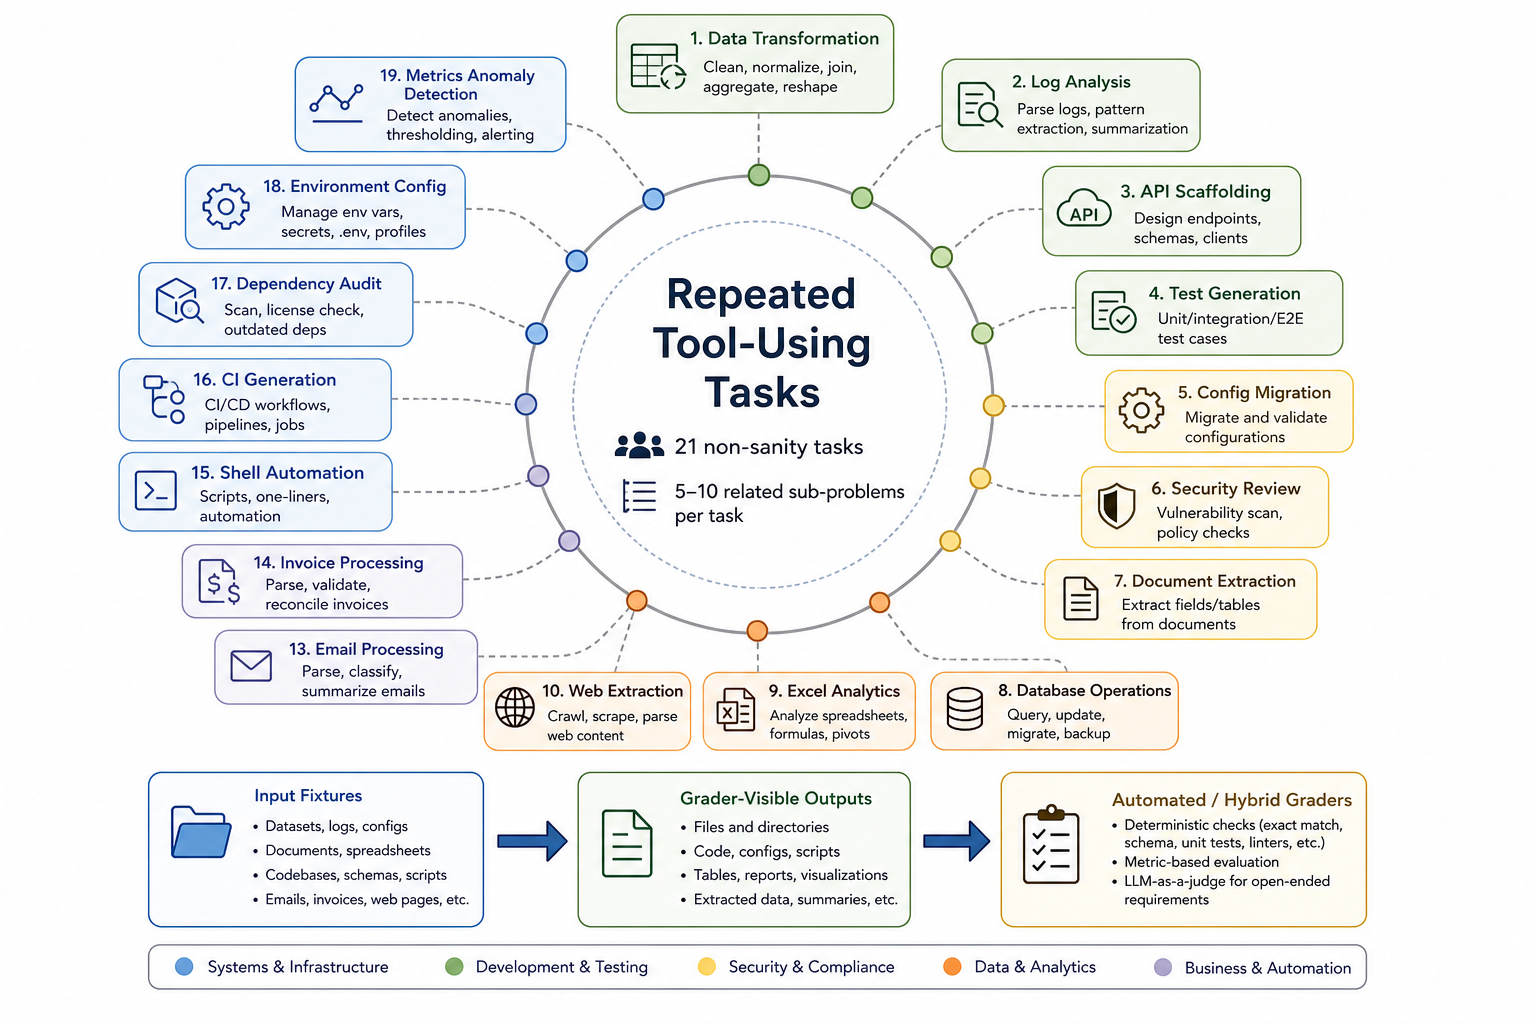
\includegraphics[width=0.94\textwidth]{Figures/fig_task_taxonomy_imagegen.png}
\caption{Task-suite structure in \ours{}. Tasks are organized around repeated tool-using sub-problems: input fixtures are copied into isolated workspaces, agents produce grader-visible artifacts, and automated or hybrid graders evaluate the resulting files.}
\label{fig:task-taxonomy}
\end{figure*}

\subsection{Workspace and Fixtures}
\label{subsec:workspace}

Each task run receives an isolated workspace.
Input assets are copied from the benchmark's fixture directory into the workspace, and the agent must write grader-visible outputs under the expected output paths.
This setup avoids relying on conversation-only answers and encourages concrete artifacts such as JSON files, scripts, reports, Dockerfiles, CI files, and structured extraction outputs.

The benchmark supports both local subprocess execution and Docker-based execution.
For reported experiments, we use local subprocess execution through the OpenClaw runtime, set \texttt{--environment local}, run 32 workers, and execute one benchmark run per task and mode.
No Docker resource limit is applied in these local runs.

\subsection{Skill Authoring and Reuse}
\label{subsec:skills}

\ours{} uses the standard \texttt{SKILL.md} format adopted by the supported runtimes.
During skill-authoring phases, the workspace is seeded with a \texttt{skill-creator} bundle that instructs the agent how to create a well-formed skill.
Generated skills are scanned from the workspace and copied into fresh execution workspaces for reuse.

To prevent a reuse run from becoming another authoring run, \ours{} hashes all non-seeded skill files before and after execution.
If a reuse execution adds, deletes, or edits a skill, the benchmark records a \texttt{skill\_mutation\_violation}.
This guardrail makes the experimental condition explicit: \preskill{} and \postskill{} execution may use generated skills, but may not improve those skills while solving the task.

\subsection{Runtimes}
\label{subsec:runtimes}

\ours{} currently supports OpenClaw and nanobot.
OpenClaw is invoked through \texttt{openclaw agent --message}, while nanobot is invoked through \texttt{nanobot run --message}.
The runtime abstraction keeps task prompts, workspaces, grading, and metrics shared across claws, allowing the benchmark to compare the same model under different agent scaffolds.
Additional runtimes can be added by implementing the same execution interface and usage extraction logic.

\section{Evaluation Protocol}
\label{sec:protocol}

\begin{figure*}[t]
\centering
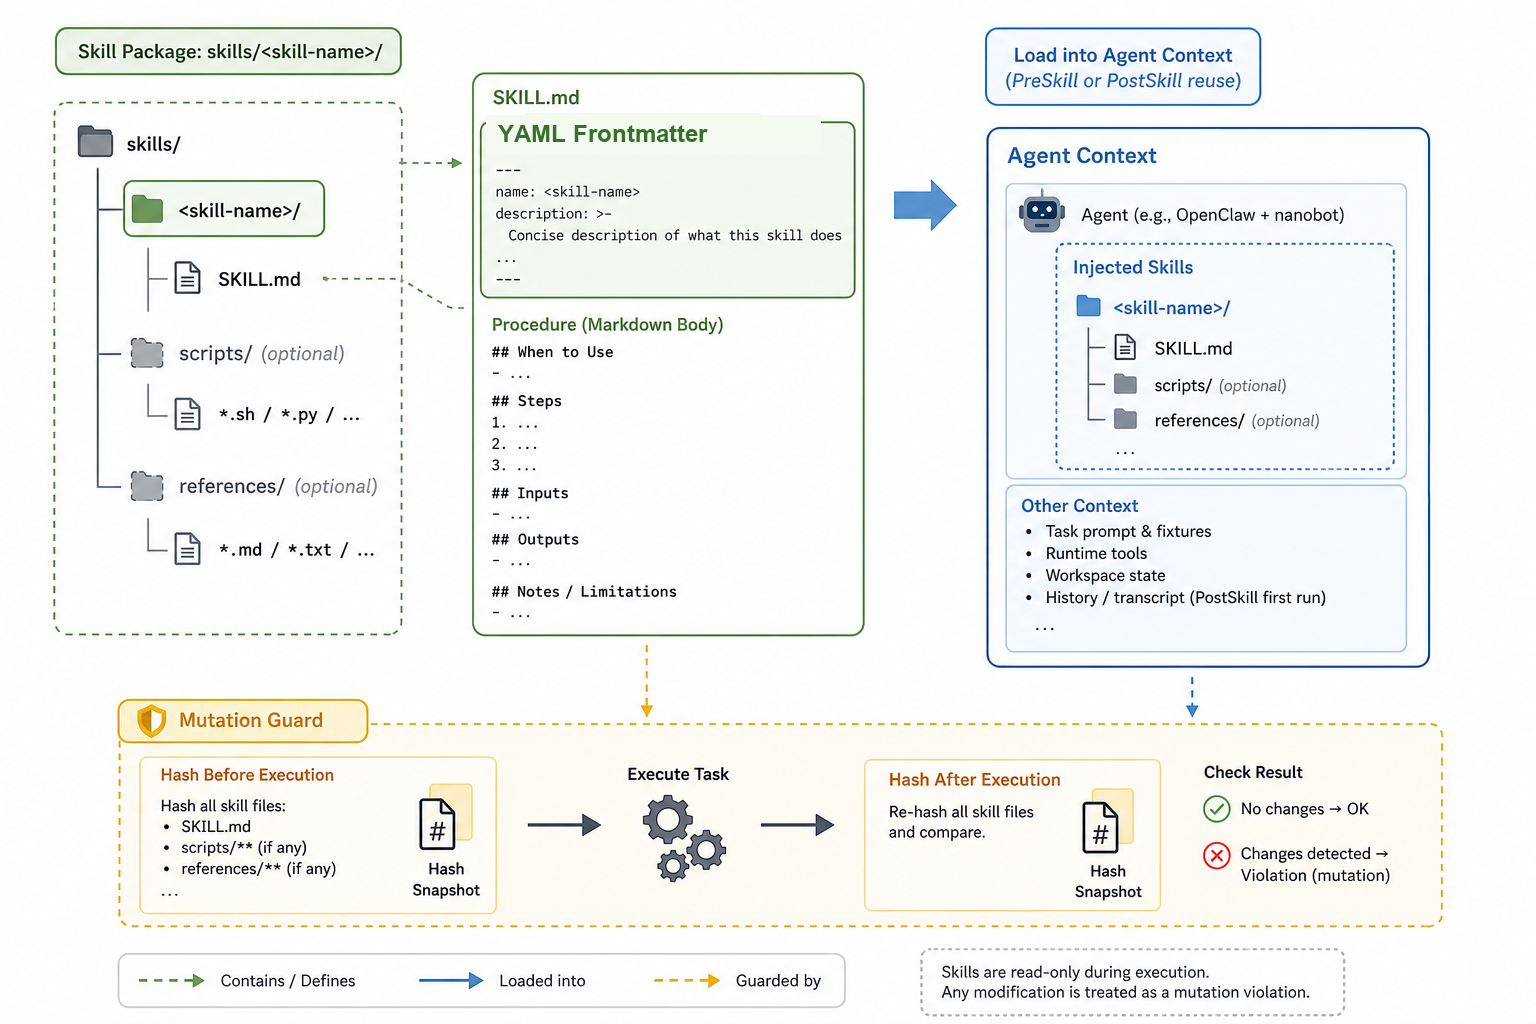
\includegraphics[width=0.86\textwidth]{Figures/fig_skill_anatomy_imagegen.png}
\caption{Structure of a reusable skill artifact in \ours{}. Generated skills use a \texttt{SKILL.md} document with optional supporting scripts or references, are injected into the agent context during reuse, and are protected by before/after mutation checks during execution.}
\label{fig:skill-anatomy}
\end{figure*}

\subsection{Three Execution Strategies}
\label{subsec:modes}

For a task $t$, model $m$, and runtime $r$, \ours{} evaluates three strategies.

\paragraph{\baseline{}.}
The agent receives the task prompt and solves it directly.
The prompt prefix forbids creating, editing, or deleting skills.
This condition measures the agent's direct task-solving ability.

\paragraph{\preskill{}.}
The agent first enters a skill-authoring phase.
It reads the skill-creator bundle and writes one or more task-specific skills under \texttt{skills/<skill-name>/SKILL.md}.
The final task outputs are not graded during this phase.
The benchmark then creates a fresh workspace, copies the generated skills into it, and runs the task execution phase with skill mutation disabled.

\paragraph{\postskill{}.}
The agent first solves the task in a no-skill execution phase.
The benchmark writes a compact \texttt{.evoclawbench/first\_run\_context.json} file containing the task prompt, grading details, output summaries, and transcript summaries.
The same runtime and model then summarize reusable skills from that first-run evidence.
A fresh second workspace executes the same task using the summarized skills.

\subsection{Metrics}
\label{subsec:metrics}

Let $S_b(t)$, $S_p(t)$, and $S_q(t)$ denote the mean task scores for \baseline{}, \preskill{}, and \postskill{}, respectively.
The primary execution-only ratios against baseline are:
\begin{equation}
    R_p(t) = \frac{S_p(t)}{S_b(t)}, \qquad
    R_q(t) = \frac{S_q(t)}{S_b(t)}.
\end{equation}
When the baseline score is zero, positive candidate scores are reported as infinite improvement and zero-to-zero comparisons are reported as $1.0$.

\ours{} reports two metric scopes.
\textbf{Execution-only} compares only the task execution phases: direct baseline execution, preskill reuse execution, and postskill second execution.
\textbf{End-to-end} includes all workflow cost: skill generation for \preskill{}, first execution and skill summary for \postskill{}, and direct execution for \baseline{}.

For each scope, the benchmark reports token, cost, and time usage.
Given baseline usage $U_b$ and candidate usage $U_x$, efficiency gain is computed as:
\begin{equation}
    E_x = \frac{U_b}{U_x}.
\end{equation}
Values greater than $1.0$ indicate that the skill workflow uses fewer resources than baseline.
The benchmark also reports created-skill counts, heuristic skill quality, and skill mutation violations.

\section{Results}
\label{sec:results}

\subsection{Experimental Setup}
\label{subsec:setup}

We evaluate three OpenClaw model runs on the hardened benchmark suite using local subprocess execution.
All runs use \texttt{uv run scripts/benchmark.py --runtime openclaw --mode all --workers 32 --environment local}; hybrid grading uses \texttt{openai/MiniMax/MiniMax-M2.7} as the judge.
Each task is run once per mode.
Unless otherwise stated, results report the execution-only mean over the benchmark loader's 101 tasks, which include the 100 official tasks plus \texttt{task\_00\_sanity}.
The numerical results in \Cref{tab:main-results} are read from the repository-local benchmark JSON files under \texttt{evoclawbench/results/}.
Rows with LLM judge failures are retained for auditability but excluded from capability conclusions.

\begin{table*}[t]
\centering
\small
\caption{Repository-local \ours{} results from current OpenClaw three-mode JSON outputs. Scores are execution-only mean task scores in percent. The loader reports 101 tasks because it includes \texttt{task\_00\_sanity} in addition to the 100 official tasks.}
\label{tab:main-results}
\resizebox{\textwidth}{!}{
\begin{tabular}{lllrrrrll}
\toprule
\textbf{Runtime} & \textbf{Model} & \textbf{Tasks} & \textbf{\baseline{}} & \textbf{\preskill{}} & \textbf{\postskill{}} & \textbf{Skills} & \textbf{Judge Failures} & \textbf{Status} \\
\midrule
OpenClaw & \texttt{openai/gpt-5.4} & 101 & 18.63 & 18.07 & 1.14 & 22 / 0 & 0 & Valid \\
OpenClaw & \texttt{openai/qwen3.6-plus} & 101 & 19.16 & 17.38 & 19.12 & 21 / 22 & 0 & Valid \\
OpenClaw & \texttt{openai/deepseek-v4-pro} & 101 & 19.99 & 15.06 & 0.00 & 21 / 0 & 13 & Invalid$^\dagger$ \\
\bottomrule
\end{tabular}
}
\vspace{0.25em}
\begin{flushleft}
\footnotesize Source files: \texttt{0061\_openai-gpt-5-4\_openclaw.json}, \texttt{0062\_openai-qwen3-6-plus\_openclaw.json}, and \texttt{0063\_openai-deepseek-v4-pro\_openclaw.json}. Slash-separated skill counts are reported as \preskill{} / \postskill{}. $^\dagger$The DeepSeek row is invalid for capability analysis because 13 LLM judge failures were observed; it is retained only to document the failure mode.
\end{flushleft}
\end{table*}

\subsection{Evaluation Findings}
\label{subsec:findings}

\paragraph{Finding 1: The hardened suite avoids baseline saturation.}
In both valid model runs, direct \baseline{} performance remains below 20\%: 18.63 for \texttt{openai/gpt-5.4} and 19.16 for \texttt{openai/qwen3.6-plus}.
This is the intended regime for evaluating skill self-evolution.
The tasks are no longer solved by simply copying exposed answer fields or following shallow schemas; agents must reconcile multi-record evidence, conflicts, revisions, and grader-visible output constraints.
As a result, a generated skill must improve a difficult execution setting rather than merely preserve performance on an already saturated benchmark.

\paragraph{Finding 2: Skill timing is model-dependent rather than monotonic.}
\texttt{openai/gpt-5.4} falls from 18.63 under \baseline{} to 18.07 under \preskill{} and 1.14 under \postskill{}.
For this model, experience-derived skills are especially brittle: the second pass nearly collapses.
\texttt{openai/qwen3.6-plus} shows a different pattern: \preskill{} falls to 17.38, while \postskill{} reaches 19.12 and nearly matches its 19.16 \baseline{} score.
These valid rows do not support a blanket claim that \preskill{} consistently outperforms \postskill{}, or that either skill workflow reliably improves over direct execution.

\paragraph{Finding 3: Skill workflows still add substantial overhead.}
Even when execution-only quality is similar, skill workflows include authoring or summarization phases.
For \texttt{openai/qwen3.6-plus}, end-to-end token-efficiency ratios are 0.38 for \preskill{} and 0.30 for \postskill{}, meaning the full workflows use substantially more tokens than direct \baseline{} execution.
For \texttt{openai/gpt-5.4}, \preskill{} has an end-to-end token-efficiency ratio of 0.36, while \postskill{} token efficiency is unavailable because the source JSON reports zero postskill tokens for that run.
The current evidence therefore suggests that self-evolution must be selective: skill creation needs to clear both a quality bar and an amortized-cost bar.

\paragraph{Finding 4: Invalid judge-failure rows must be separated from capability claims.}
\texttt{openai/deepseek-v4-pro} reports 19.99 under \baseline{}, 15.06 under \preskill{}, and 0.00 under \postskill{}, but the run contains 13 LLM judge failures.
We therefore do not interpret the 0.00 \postskill{} score as model incapability.
Instead, it marks a benchmark infrastructure failure mode: hybrid-graded runs can become invalid when judge calls fail, and result tables must carry validity metadata rather than silently mixing invalid rows into aggregate conclusions.

\begin{figure*}[t]
\centering
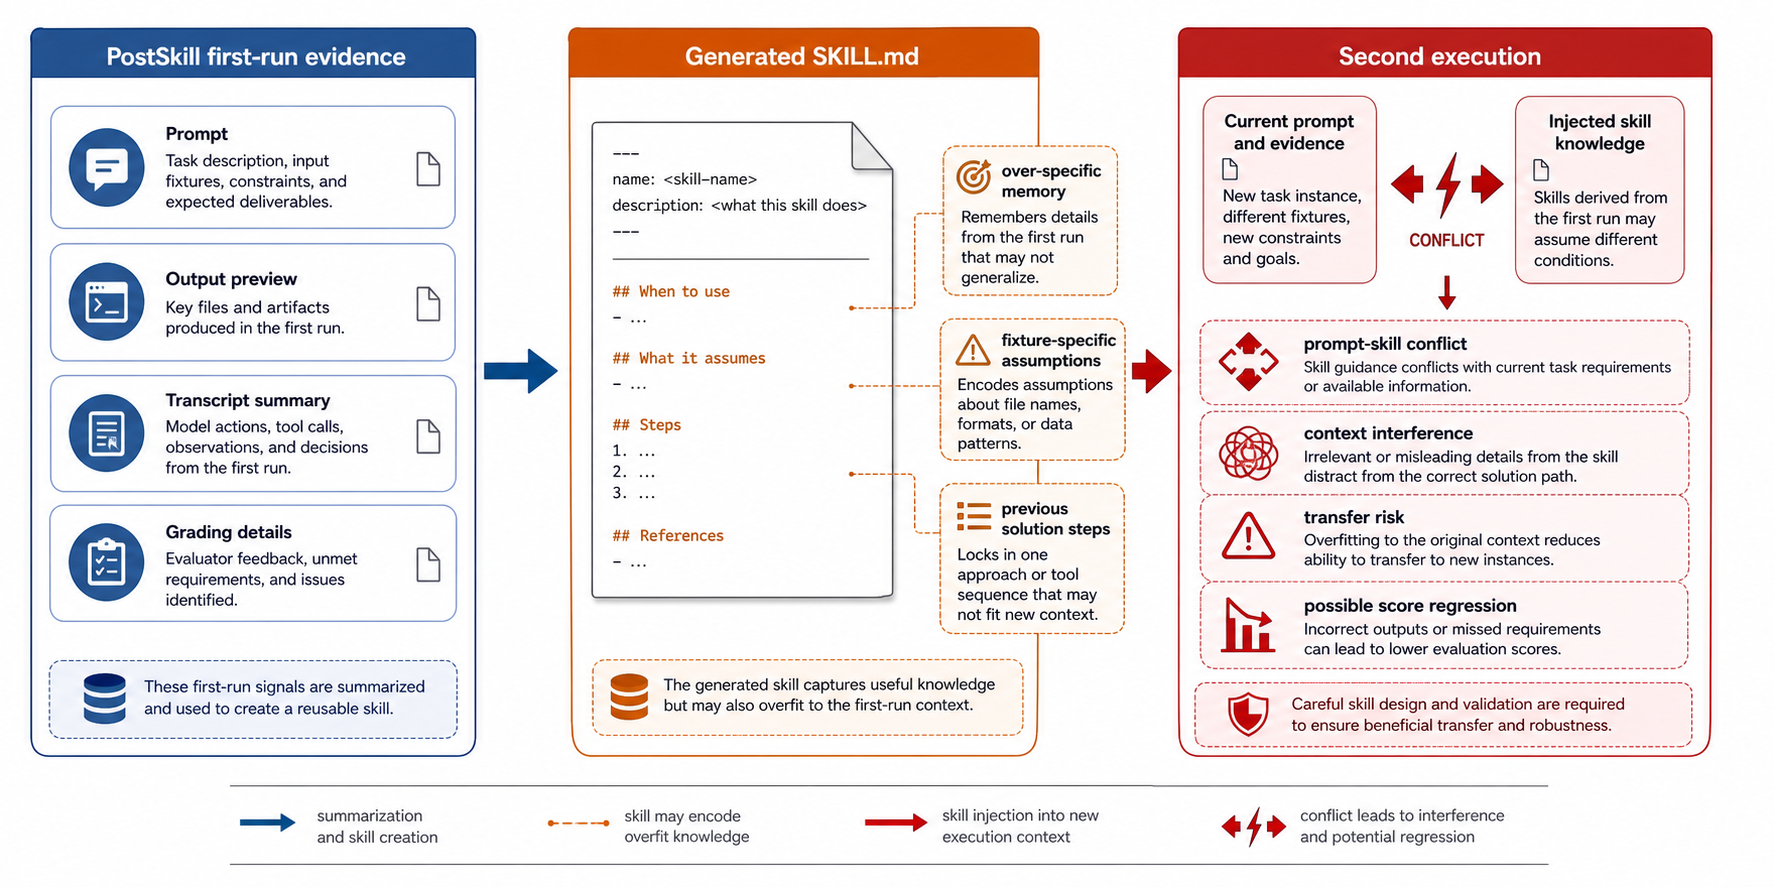
\includegraphics[width=\textwidth]{Figures/fig_failure_case_imagegen.png}
\caption{Qualitative failure mode for experience-derived skills. In \postskill{}, first-run evidence can help produce reusable procedural memory, but it can also encode over-specific assumptions that interfere with the second execution context.}
\label{fig:failure-case}
\end{figure*}

\section{Discussion}
\label{sec:discussion}

\ours{} reframes skill evaluation around the full lifecycle of procedural memory.
A deployed agent does not only receive curated skills from a user.
It may decide that a task is repetitive, write a new skill, use the skill immediately, and later update a skill library.
Our results suggest that current agents are not yet reliable at this lifecycle.

The current hardened results put this lifecycle in a low-score regime rather than a saturated one.
That makes the negative and mixed skill results more informative: the agents have room to improve, but the self-authored skill phases do not reliably convert repeated structure into higher task scores.
\preskill{} asks the agent to infer an abstract procedure from repeated sub-problems before committing to a concrete solution, while \postskill{} adds evidence from a completed run.
The valid runs show that neither strategy is uniformly dominant across models.
First-run evidence can sometimes preserve baseline-like behavior, as in \texttt{openai/qwen3.6-plus}, but it can also interfere with the second execution, as in \texttt{openai/gpt-5.4}.

These observations imply that future skill systems should treat self-evolution as a selective operation rather than a default behavior.
Agents may need confidence estimates for whether a task is worth skill creation, a preference for \preskill{}-style authoring when skill creation is warranted, validation checks for generated skills, and policies that decide when a skill should be reused, revised, or discarded.

\section*{Limitations}

The current v1 protocol evaluates \postskill{} by rerunning the same task with the same fixtures, which measures within-task skill distillation but does not yet test transfer to unseen related tasks.
The task suite covers many practical office, data, coding, DevOps, and security workflows, but it is still smaller than large public agent benchmarks.
Hybrid grading tasks may depend on the selected judge model, although automated checks are used whenever feasible.
The current reported table has two valid model rows and one invalid audit row; additional planned MiniMax and GPT-5.4-mini runs were not completed under a failure-free judge path and are therefore not included as result rows.
Finally, the current implementation supports OpenClaw and nanobot, but the reported experiments here cover only OpenClaw; broader runtime coverage is needed before claiming conclusions across all major claw frameworks.

\section*{Acknowledgments}

Omitted for anonymous review.

\bibliography{references}

\appendix

\section{Prompt Prefixes}
\label{app:prefixes}

\ours{} controls each mode with explicit prompt prefixes.
\baseline{} forbids creating, editing, or deleting skills.
\preskill{} first asks the agent to create task-specific skills under \texttt{skills/<skill-name>/SKILL.md}, then runs a fresh skill reuse phase.
\postskill{} first executes the task, writes first-run context, asks the agent to summarize reusable skills, and then executes the task again with the summarized skills.

\section{Skill Artifact Structure}
\label{app:skill-artifact}

\begin{figure*}[t]
\centering
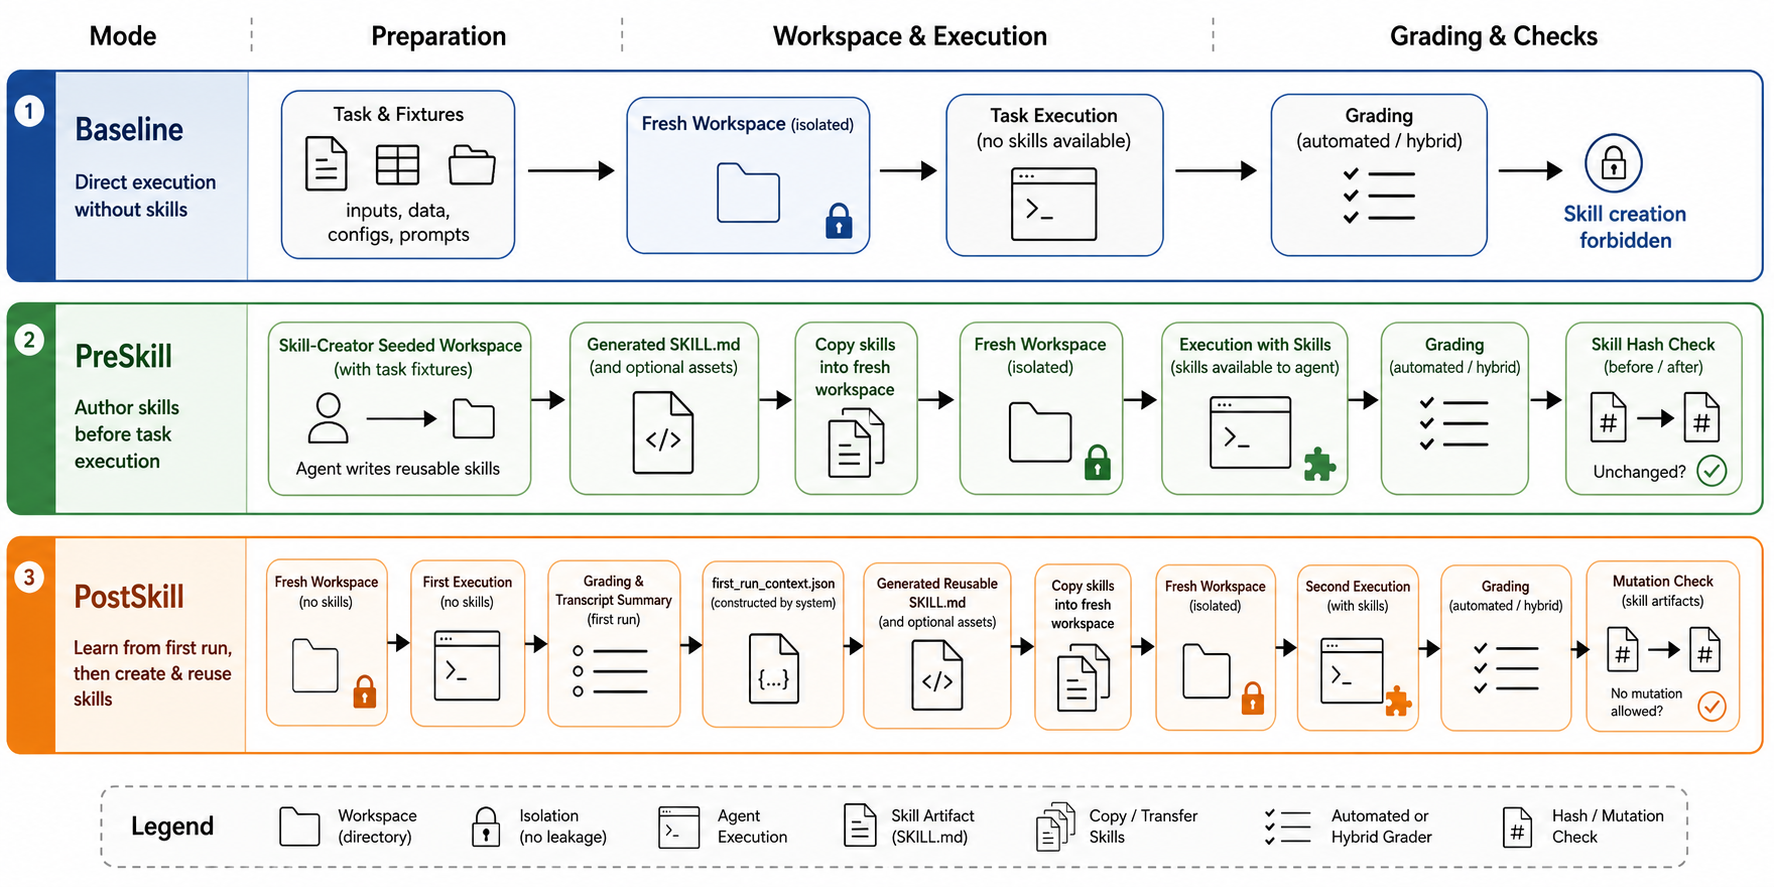
\includegraphics[width=\textwidth]{Figures/fig_protocol_imagegen.png}
\caption{Three-mode evaluation protocol. \baseline{} directly executes a task without skill creation; \preskill{} first creates task-specific skills and then reuses them in a fresh workspace; \postskill{} summarizes reusable skills from first-run evidence before a second execution. Skill reuse phases are checked for mutation violations.}
\label{fig:protocol}
\end{figure*}

\section{Result JSON Schema}
\label{app:json}

The aggregate output JSON contains \texttt{baseline\_results}, \texttt{preskill\_results}, \texttt{postskill\_results}, and \texttt{metrics}.
The \texttt{metrics} object contains \texttt{execution\_only}, \texttt{end\_to\_end}, \texttt{postskill}, \texttt{created\_skills}, \texttt{skill\_quality}, and \texttt{skill\_mutation\_violations}.

\section{Result Validity Checklist}
\label{app:checklist}

Before adding a result row, record the source JSON file, model, runtime, mode, environment, worker count, judge model, loaded task count, official task count, mean scores for all modes, created-skill counts, mutation violations, and judge-failure count.
Runs with any LLM judge failure should be labeled as invalid or audit-only and should not be used for model-capability conclusions until rerun successfully.

\end{document}
